\documentclass{SGGW-thesis-EN}
\usepackage[utf8]{inputenc}
\usepackage[backend=biber,style=numeric]{biblatex}
\usepackage{tabularx}
\usepackage{tikz}
\usetikzlibrary{positioning, arrows.meta, shapes.geometric}
\addbibresource{references.bib}

\MASTERtrue
\WZIMtrue

\title{Automated Extraction and Categorization of Product Information from Receipts}
% command \Ptitle{} can be used to give the title in Polish, if this is necessary, and can be deleted if you do not need the title in Polish
\Ptitle{}
\author{Michał Zaręba}
\date{2017}
\album{196218}
\thesis{Diploma thesis in the field of}
\course{Information Science}
\promotor{dr hab.\ inż.\ Leszek Chmielewski, prof.\ SGGW}
\pworkplace{Institute of Information Technology\\Department of Artificial Intelligence}

\usepackage{hyperref}

\begin{document}
\maketitle
\statementpage
% titles and abstracts must be given in two languages - PL, EN
\abstractpage
{OCR + BERT}
{Tematem niniejszej pracy było zaimplementowanie klasy \LaTeX{}owej pozwalającej na formatowanie tekstu zgodnie z wytycznymi nałożonymi przez uczelnię. Praca zawiera dwie
główne części. Pierwsza z nich zawiera opis najważniejszych aspektów implementacji klasy. Natomiast druga część skupia się na sposobie użycia klasy przez osoby piszące prace
dyplomowe.}
{OCR, BERT, Tesseract, thesis, implementation, SGGW, Warsaw University of Life Sciences}
{OCR + BERT}
{The subject of this thesis was to implement a \LaTeX{} class that allows formatting text according to the guidelines imposed by the university. The thesis contains two main}
{LaTeX, class, thesis, implementation, SGGW, Warsaw University of Life Sciences}



\tableofcontents


\startchapterfromoddpage % niezależnie od długości spisu treści pierwszy rozdział zacznie się na nieparzystej stronie

\chapter{Introduction}

\section{Motivation}
Tracking of expenses and managing personal finances is an important aspect of modern life.
With an increasing number of daily transactions and a vast variety of products available, individuals face significant challenges in effectively monitoring their spending and managing their budgets. 
Although receipts contain valuable details that could help consumers analyze and control their expenses, 
the majority of consumers either discard receipts shortly after purchase or find it too tedious and time-consuming to analyze them manually. 
Automating the extraction and categorization of product information from receipts could significantly simplify budget tracking and provide insights into spending habits, enabling consumers to understand precisely where their money goes.
Simple and efficient way to track expenses is essential for individuals who wish to maintain a clear overview of their spending habits and make informed financial decisions. 


\section{Problem Statement}
Most existing expense-tracking solutions focus primarily on invoices, bank statements, or require manual input. 
Large corporations and organizations typically possess the necessary budgets and technical resources to implement robust, 
automated systems for extracting and categorizing expense data from structured documents such as invoices or bank statements. 
For personal use, however, the most commonly available and practical source of spending information remains paper receipts. 
Current receipt-based solutions are often limited: many tools available today are either designed exclusively for commercial purposes, 
lack support for languages other than English, or are inadequately trained to accurately process Polish-language receipts.  
Thus, there is a clear gap and a significant need for a solution that effectively automates extraction and categorization of product details from receipts, 
specifically accommodating the complexity and linguistic characteristics of the Polish language.

\section{Objectives of the Study}
This study has two primary objectives, each directly addressing the challenges identified in the problem statement:

\begin{enumerate} 
  \item Develop a robust system capable of automatically extracting structured product information (such as product names, and prices) from Polish-language receipts using Optical Character Recognition (OCR).
  \item Implement and evaluate a product categorization module based on the embeddings generated by pre-trained models, specifically BERT (Bidirectional Encoder Representations from Transformers),
  and Sentence-BERT model (Siamese transformer network) fine-tuned with own data. 
  \item The extracted embeddings serve as input to an XGBoost classifier responsible for categorizing products into predefined expense-related categories.
\end{enumerate}

These objectives will be thoroughly addressed and analyzed in subsequent chapters. 
Given the complexity of Polish-language receipts and limited availability of labeled datasets, achieving optimal results will require careful integration and fine-tuning of multiple technologies. 
Critical aspects will include the effective integration of OCR and NLP components, as well as the development of a robust classification model capable of accurately categorizing products based on their textual descriptions that might
often be ambiguous, multiple-worded, or contain spelling errors.
\newpage
\section{Scope and Limitations}

The scope of this study is limited to the development of a system capable of automatically extracting product information from receipts and categorizing these products into predefined categories. 
The system specifically targets Polish-language receipts and will be evaluated primarily on its ability to accurately extract product costs and perform correct product categorization.

\noindent \\The limitations of this study include the following:

\begin{itemize}
    \item The developed system will not include additional functionalities such as expense tracking over time, financial report generation, or integration with external personal financial management tools.
    \item The scarcity of comprehensive, labeled Polish-language receipt datasets restricts the potential accuracy and generalization capabilities of the models developed. Consequently, results may vary when encountering receipt formats or text variations not present in the training data.
    \item The OCR will be employed without utilizing spatial information or context regarding the positioning of text on receipts. Therefore, preprocessing steps such as image cropping, alignment, and noise reduction are necessary to ensure the OCR engine receives properly formatted and isolated textual inputs.
\end{itemize}

\chapter{Literature Review}

\section{Optical Character Recognition (OCR) Technologies}
Optical Character Recognition (OCR) refers to the process of converting textual information from scanned or photographed images into machine-readable formats. 

Traditional OCR techniques primarily relied on template matching, statistical classification, and structural analysis, with limited adaptability to varying fonts and noisy inputs.\cite{ocrsystems}

Modern OCR systems use deep learning models that typically combine convolutional neural networks (CNNs) for feature extraction with recurrent or attention-based architectures (e.g., LSTM, GRU) for sequence modeling. This architecture enables the system to learn complex patterns and recognize characters across varying fonts, sizes, and orientations \cite{shi2016endtoend}.

Recent OCR models further incorporate attention mechanisms, allowing the network to dynamically focus on relevant regions of the input image. Unlike standard OCR models, LayoutLM introduces explicit spatial awareness by incorporating positional embeddings of text regions, which is particularly effective for structured documents like receipts \cite{li2020layoutlm}.
While attention-based models with spatial awareness offer notable improvements in accuracy and robustness, their effectiveness remains constrained by the availability of large, annotated datasets. As a result, the OCR systems evaluated in this study—Tesseract and PaddleOCR—do not model document structure explicitly and operate at the text-line level.

Tesseract is an open-source OCR engine maintained by Google, widely adopted across various applications. It supports multiple languages, including Polish, and can be fine-tuned on domain-specific datasets for improved accuracy. Since version 4.0, it incorporates an LSTM-based recognition engine, enhancing its performance on noisy or multilingual documents \cite{smith2007overview, smith2013history}. Tesseract is highly configurable, offering control over segmentation modes, character whitelists, and language models. Fine-tuning involves training on a targeted dataset, which can significantly enhance accuracy for specific formats such as Polish receipts.
\newpage
PaddleOCR is a deep learning-based OCR framework developed by Baidu, supporting over 80 languages. The framework proposes a OCR system,
that is modular and made of text detection, detected boxes rectification and text recognition. Thanks to the use of a several augmentation techniques, PaddleOCR achieves a balance between accuracy and speed, 
making it suitable for real-time applications and mobile devices.

Text detection is handled using Differentiable Binarization that is a segmentation network. Simplicity of the model combined with minor postprocessing
holds the effectiveness of this module. Then the detected boxed are rectified using a text direction classifier and fed into a text recognition model.
The text recognition model is based on a CRNN architecture, specifically designed for recognizing characters in images. 
It employs a combination of convolutional layers and recurrent layers to capture both local and sequential features of the text. 
For further enchancement several strategies are used, such as light backbone or data augmentation \cite{du2020ppocr}. 

\begin{figure}[h!]
  \centering
  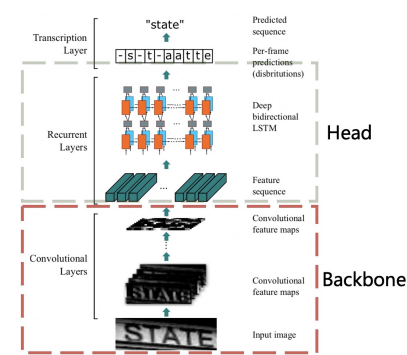
\includegraphics[width=1\textwidth]{images/cnn_text_recognizer.png}
  \caption{CRNN text recognition architecture. \cite{shi2015e2etnn}}
  \label{fig:cnn_text_recognizer}
  \end{figure}
\begin{figure}[h!]
  \centering
    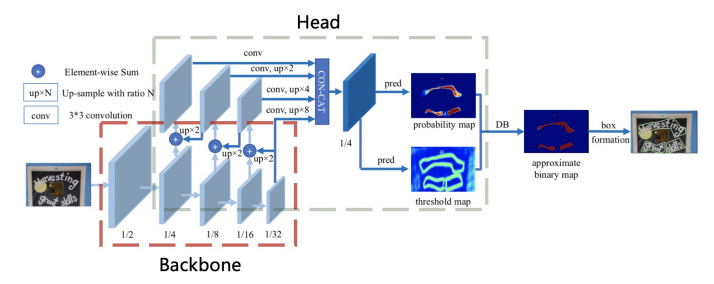
\includegraphics[width=1\textwidth]{images/text_detector_db.png}
    \caption{DBNet text detection architecture. \cite{liao2019rttextdet}}
    \label{fig:text_detector_db}
  \end{figure}

\newpage
\section{Semantic Text Embeddings for Receipt Item Categorization}
To enable machine learning models to analyze text, the text must first be converted into a numerical format—a process known as vectorization or word embedding which is a crucial step in Natural Language Processing (NLP).
Word embeddings are fixed-length vector representations that encode the semantic meaning of words and the relationships between them. 
The words with similar meanings are represented by similar vectors in the embedding space.\cite{almeida2023wordembeddingssurvey}

\begin{figure}[h!]
  \centering
    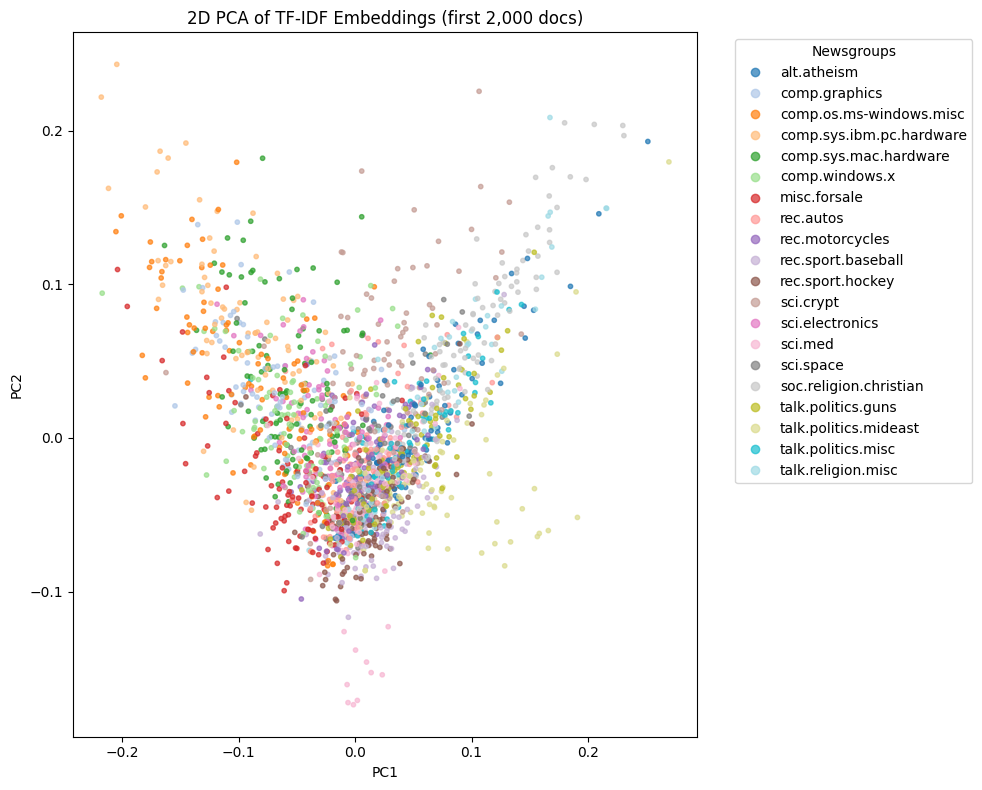
\includegraphics[height=9cm]{images/tfidf_embeddings.png}
    \caption{TF-IDF embeddings on News Groups dataset from scikit-learn.}
    \label{fig:tfidf_embeddings}
  \end{figure}

\newpage 
There are several approaches to generating these embeddings, and this section outlines the most common methods, explaining how they work and highlighting their key differences.
Prior to embedding, text must be preprocessed. This includes normalization steps such as lemmatization or stemming, and tokenization, which segments text into individual words or tokens \cite{jurafsky2023slp3}.
After those we can proceed to several methods of generating word embeddings, which can be broadly categorized into two groups: count-based and prediction-based methods, and will be described below.

\subsection{Count-based Methods}
Count-based methods rely on the idea that the meaning of a word can be inferred from its co-occurrence with other words in a given context.
Those methods typically involve creating a sparse matrix, where each row and column represents a word in the vocabulary, and the values in the matrix represent the frequency of co-occurrence between pairs of words.
The two most common approaches are the Bag of Words (BoW) and Term Frequency-Inverse Document Frequency (TF-IDF)\cite{jurafsky2023slp3}.

Bag of words represents a document as an unordered vector of word counts, ignoring the order of words and their grammatical relationships.

TF-IDF model, on the other hand, assigns weights to words based on their frequency in a document relative to their frequency in the entire corpus. 
This helps to highlight important words that are more informative for the specific document.

\subsection{Prediction-based Methods}
Prediction-based methods are word representation techniques that learn embeddings by predicting words from context (or vice versa), unlike count-based methods which rely on raw frequency statistics.
The two most common prediction-based methods are Word2Vec and BERT which are based on neural networks and their representation of words is contained in dense matrix different from the sparse matrix used in count-based methods.
The dense matrixes turns out to be more efficient and effective for representing the meaning of words in a lower-dimensional space.\cite{jurafsky2023slp3}

Word2vec is a framework used for calculating a static embeddings, that mean there is a certain numerical representation for each word in vocabulary.
There are two architectures for training Word2Vec models: Continuous Bag of Words (CBOW) and Skip-Gram.
\begin{enumerate}
  \item \textbf{Continuous Bag of Words (CBOW)}: predicts the target word from surrounding context words.
  \item \textbf{Skip-Gram} Skip-Gram: predicts context words from a single target word.
\end{enumerate}
Skip-Gram is particularly effective for representing rare words, as it captures word–context associations more accurately,
whereas CBOW offers greater computational efficiency and faster training times \cite{mikolov2013distributed}.

\textbf{BERT (Bidirectional Encoder Representations from Transformers)} is a deep learning model introduced by Google that generates contextualized word embeddings by processing text in both directions (left-to-right and right-to-left) simultaneously. 
Unlike earlier models that produce static embeddings, BERT captures the meaning of a word based on its entire sentence context. 
Transformer architecture, the backbone of BERT, employs self-attention mechanisms to weight the importance of words in relation to each other, allowing the model to derivate complex semantic relationships between them.
To achieve this, BERT is pretrained using a two-step self-supervised training process:
\begin{enumerate}
  \item \textbf{Masked Language Model (MLM)}: Randomly masks a percentage of input tokens and trains the model to predict the masked words based on context.
  \item \textbf{Next Sentence Prediction (NSP)}: Trains the model to predict whether two sentences are follow each other or not, improving its understanding of sentences coherence.
\end{enumerate}

\begin{figure}[h!]
  \centering
    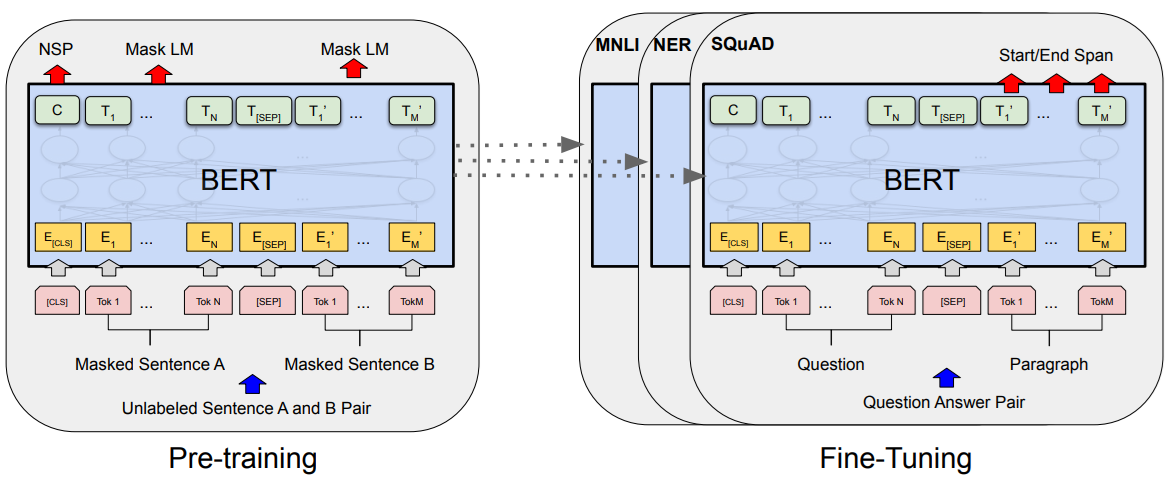
\includegraphics[height=5cm]{images/bert_procedures.png}
    \caption{BERT training procedures \cite{devlin2019bertpretrainingdeepbidirectional}}
    \label{fig:bert_procedures}
  \end{figure}

These context-aware embeddings have demonstrated strong performance across various NLP tasks, including classification.\cite{devlin2019bertpretrainingdeepbidirectional}.
In this study, embeddings generated by pre-trained BERT models serve input features for classification task which will categorize products into predefined expense-related categories.


\section{XGBoost Classifier}
XGBoost (eXtreme Gradient Boosting) is an open-source machine learning library implementing the gradient boosting framework, 
primarily with decision trees. It is a state-of-the-art supervised learning algorithm known for consistently achieving top performance across numerous machine learning challenges \cite{Chen_2016}.

Gradient boosting is an ensemble learning technique that instead of training a single model, build an initial simple model 
and then iteratively fits new models to  minimize the loss function\cite{natekin2013gradient}.

The XGBoost model employs several specific techniques to enhance its predictive capabilities:
\begin{enumerate}
  \item Regularization: Prevents the creation of overly complex trees, thereby minimizing overfitting and improving generalization.
  \item Gradient Tree Boosting with second-order Taylor approximation: Incorporates both first-order (gradient) and second-order (Hessian) derivatives of the loss function, significantly improving estimation accuracy and computational efficiency.
  \item Shrinkage (learning rate): After each boosting step, prediction scores are scaled by a small factor (learning rate). This regularization strategy prevents overfitting and ensures the model learns gradually and robustly.
  \item Column subsampling: Inspired by random forests, this technique randomly selects subsets of features when building each tree, further reducing overfitting and enhancing training efficiency. 
\end{enumerate}
XGBoost uses an ensemble of decision trees to make predictions. 
Each tree in this ensemble contributes to the final prediction by adding its own output to the outputs of all previous trees.

Mathematically, the final prediction $\hat{y}_i$ for an instance $x_i$ is given by:

\begin{figure}[h!]
  \centering
  \begin{minipage}[c]{0.4\textwidth}
      \centering
      \[
      \hat{y}_i = \sum_{k=1}^{K} f_k(x_i)
      \]
  \end{minipage}\hfill
  \begin{minipage}[c]{0.55\textwidth}
      \centering
      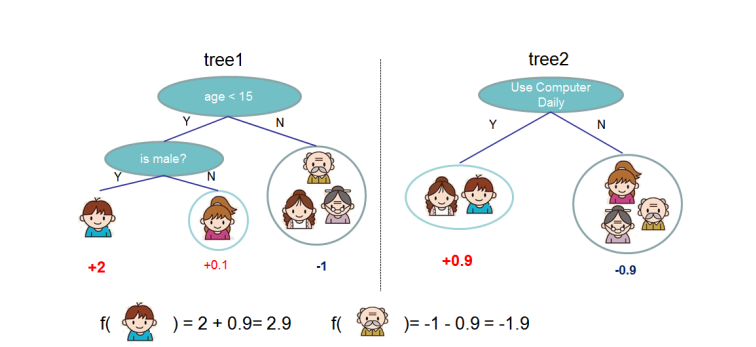
\includegraphics[width=\linewidth]{images/tree_ensemble_model.png}
      \caption{Tree ensemble model \cite{Chen_2016}}
      \label{fig:tree_ensemble_model}
  \end{minipage}
\end{figure}
To train these trees effectively, XGBoost optimizes a simplified objective function derived using second-order approximations (gradients and Hessians). 
This objective helps determine the optimal structure and weights of each tree. \newpage The simplified final objective at each iteration is expressed as:

\begin{figure}[h!]
  \centering
  \begin{minipage}[c]{0.4\textwidth}
      \centering
    \[
    \tilde{L}^{(t)}(q) = -\frac{1}{2}\sum_{j=1}^{T}\frac{(\sum_{i \in I_j} g_i)^2}{\sum_{i \in I_j} h_i + \lambda} + \gamma T
    \]
  \end{minipage}\hfill
  \begin{minipage}[c]{0.55\textwidth}
      \centering
      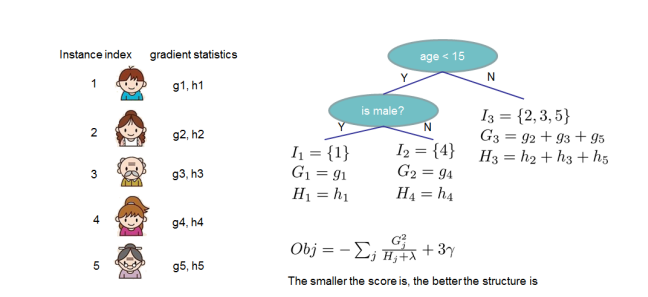
\includegraphics[width=\linewidth]{images/Structure score calculation.png}
      \caption{Structure Score Calculation \cite{Chen_2016}}
      \label{fig:Structure_score_calculation}
  \end{minipage}
\end{figure}
Here, $g_i$ and $h_i$ represent gradient statistics, indicating how predictions should change to minimize the error. The terms $\gamma$ and $\lambda$ are hyperparameters that penalize complex trees to prevent overfitting.
Hyperparameters are parameters defined before training, which control the learning process.  
In XGBoost, these hyperparameters significantly affect how the model is trained and how it performs.
\begin{table}[h!]
  \centering
  \caption{XGBoost Hyperparameters and Their Roles}
  \label{tab:xgboost_hyperparameters}
  \begin{tabularx}{\textwidth}{|l|X|}
  \hline
  \textbf{Hyperparameter} & \textbf{Role and Effect} \\ \hline
  \texttt{learning\_rate} & Controls the rate at which the model learns. Lower values reduce overfitting but require more trees. \\ \hline
  \texttt{max\_depth} & Limits the depth of the trees. Greater depth increases model complexity and the risk of overfitting. \\ \hline
  \texttt{n\_estimators} & Determines the total number of trees in the ensemble. Increasing trees usually enhances performance but extends training time. \\ \hline
  \texttt{subsample} & The fraction of samples randomly chosen to build each tree. Lower values help reduce overfitting. \\ \hline
  \texttt{colsample\_bytree} & The fraction of features randomly selected to build each tree, reducing correlations between trees and preventing overfitting. \\ \hline
  \texttt{min\_child\_weight} & Minimum sum of instance weights in a child node. Higher values encourage simpler, less detailed trees, reducing overfitting. \\ \hline
  \texttt{gamma} & Minimum required loss reduction for creating new splits. Higher values lead to simpler, more generalized models. \\ \hline
  \texttt{reg\_alpha} & L1 regularization term applied to leaf weights. Higher values increase sparsity (fewer active features). \\ \hline
  \texttt{reg\_lambda} & L2 regularization term applied to leaf weights. Larger values penalize extreme weights, preventing overfitting. \\ \hline
  \end{tabularx}
  \end{table}

Adjusting these hyperparameters influences the balance between fitting the training data closely and maintaining a simpler, more generalizable model.

\section{Challenges in OCR and NLP for Document Understanding}

The integration of OCR and NLP technologies for document understanding presents several challenges, 
particularly when dealing with complex documents such as receipts. 
These challenges include variability in receipt formats, noise and distortion in images, and language-specific characteristics. 
Even the most advanced OCR systems struggle to achieve high accuracy on low-quality images. 

Several approaches can be used to improve OCR performance, including simple image preprocessing techniques such as binarization, 
denoising, and skew correction, which enhance the quality of input images.

To further improve the understanding of extracted text, techniques such as 2D positional embeddings are employed. 
2D positional embeddings encode the spatial location of text tokens within a two-dimensional layout, such as a document or receipt. 
Unlike standard positional embeddings in sequential models, which capture only the order of tokens in one dimension (e.g., left to right), 
2D positional embeddings represent both horizontal (x-axis) and vertical (y-axis) coordinates. 
This spatial information allows models to better understand the structure of documents and improve downstream processing tasks \cite{subramani2021surveydeeplearningapproaches}.

Another method to enhance the OCR process involves using a restoration model, such as an Action Prediction Model, which aims to correct degraded text. 
The model operates by predicting correction actions for each character extracted from the OCR output. 
Applying this approach can significantly improve the performance of downstream tasks, such as Named Entity Recognition (NER), 
by refining the text before further processing. In one study, the F1 score for NER increased from 0.59 to 0.895, reducing the performance gap by 76\% \cite{gupte2021lightscameraactionframework}. 
This restoration method also shows strong potential for improving text classification tasks.

One of the most critical challenges in document understanding, particularly for OCR tasks, 
is the scarcity of labeled datasets for training and evaluation. 
Creating large datasets is difficult because each document image must be paired with accurate text annotations,
which is especially challenging for complex documents like receipts. \cite{subramani2021surveydeeplearningapproaches}
The shortage of labeled data increases the risk of overfitting, 
where models achieve high performance on training examples but generalize poorly to new, unseen documents.
On the other hand, the possibility of generating a synthetic dataset is a promising approach to overcome the lack of labeled data, 
and it can be already achievied by using a generative model such as Genalog \cite{gupte2021lightscameraactionframework} or other LLM-based models.

\chapter{Methodology}


\section{Introduction}
This chapter presents the methodology employed to develop and evaluate a system for automatically extracting product information from 
olish-language receipts and categorizing those products into expense-related classes. 
The approach comprises data acquisition, preprocessing, embedding generation, classification, and experimental evaluation. 
Project structured in a way that allows for systematic comparison of different embedding strategies and their impact
 on classification performance while also keeping the overall process scalable and adaptable to future improvements.


\section{Research Design}
The primary objective of this study is to develop and rigorously evaluate an end-to-end system for extracting and categorizing product information from receipts. 
To achieve this, the research design adopts a modular approach: each component (OCR, embedding generation, and classification) can be developed and tested independently, 
while still integrating into a unified workflow. 
This structure not only enables targeted evaluation of individual modules but also supports direct comparison across different models and techniques. 
Finally, model performance is assessed under four experimental conditions—3-class and 8-class categorization, each tested with both original and GPT-augmented training data—to measure robustness across varying levels of complexity and data composition.class), 
 with controlled variation of input features and training data composition.

The dataset used in this study is relatively small as it consists of only 20 scanned receipts, yielding a total of 263 individual line‐item entries. 
We apply a standard 70/30 train/test split, resulting in 184 entries for training and 79 entries for testing.
Polish‐specific textual challenges further complicate the task. First, diacritical marks (e.g., “ł”, “ó”, “ą”, “ę”) are frequent and, 
if misrecognized by OCR, can lead to incorrect tokenization and erroneous embeddings. 
Second, receipts often employ numerous abbreviations and shortcuts—such as “kg” for kilograms or truncated product names (ZIEL, KAJZ etc.)—
introducing high lexical variability. These factors necessitate targeted preprocessing 
(e.g., regex rules for diacritic restoration and expansion of common abbreviations) and robust embedding strategies to mitigate recognition errors and vocabulary fragmentation.

Model performance is evaluated using the macro-averaged F1 score, which balances precision and recall across all classes. 
As a baseline, I implement a straightforward pipeline comprising Tesseract OCR for text extraction, TF-IDF vectorization for feature representation, 
and a logistic regression classifier. 
This baseline enables quantification of the performance gains achieved through advanced embedding models and XGBoost classification.

\begin{figure}[h!]
  \centering
  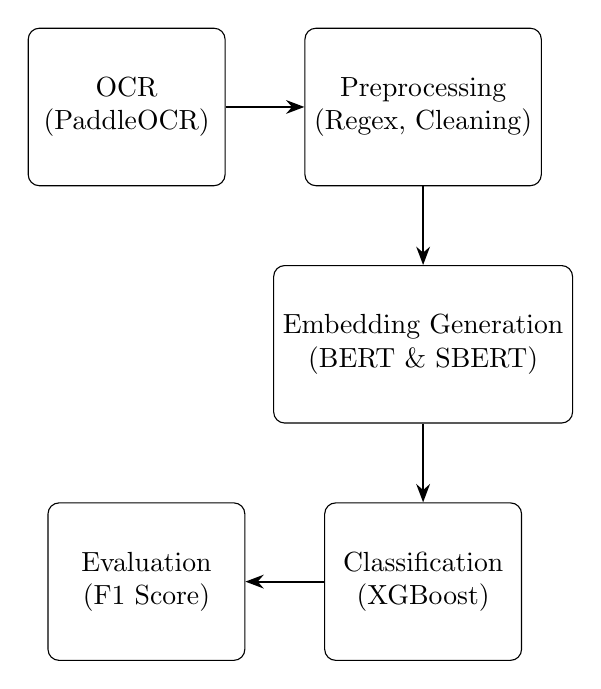
\begin{tikzpicture}[
      box/.style={
        rectangle,
        draw,
        rounded corners,
        minimum width=2.5cm,
        minimum height=2cm,
        align=center
      },
      >={Stealth},
      every edge/.style={draw, thick, -{Stealth}},
      node distance=1cm
    ]
    % Nodes
    \node[box] (ocr) {OCR\\(PaddleOCR)};
    \node[box, right=of ocr] (pre) {Preprocessing\\(Regex, Cleaning)};
    \node[box, below=of pre] (emb) {Embedding Generation\\(BERT \& SBERT)};
    \node[box, below=of emb] (clf) {Classification\\(XGBoost)};
    \node[box, left=of clf] (eval) {Evaluation\\(F1 Score)};

    % Arrows
    \path (ocr) edge (pre)
          (pre) edge (emb)
          (emb) edge (clf)
          (clf) edge (eval);
  \end{tikzpicture}
  \caption{High‐level flowchart of the receipt processing and classification pipeline}
  \label{fig:pipeline_flowchart_vertical}
\end{figure}


\section{Data Sources and Collection Procedures}
The primary data consist of textual outputs generated by applying PaddleOCR to scanned receipt images. 
To address class imbalance, supplementary synthetic examples were created using GPT-based generation techniques, ensuring more uniform category distributions.

Text was extracted from receipt images using PaddleOCR, then segmented into individual rows corresponding to line items. 
Each row was manually annotated with the correct product category label and associated cost, following a predefined annotation protocol.

\section{Data Preparation and Features}
Annotated entries were loaded into the analysis environment and category labels were encoded numerically. Text normalization was performed via regular expressions, including lowercasing, removal of extraneous symbols, and language-specific cleaning. Two types of embeddings were generated for each row:
\begin{itemize}
  \item Contextual embeddings from a pretrained Polish BERT model (\texttt{dkleczek/bert-base-polish-cased-v1}).
  \item Sentence-level embeddings from a fine-tuned Sentence-BERT model (\texttt{all-MiniLM-L6-v2}).
\end{itemize}

\section{Modeling and Analysis}


\section{Experimental Setup and Evaluation}
Experiments were managed via the Hydra framework to ensure reproducibility of configurations. Training incorporated both original and GPT-augmented data to balance class distributions. Two classification scenarios were evaluated:
\begin{enumerate}
  \item 3-class categorization  
  \item 8-class categorization  
\end{enumerate}
Model performance metrics (e.g., accuracy, F1-score) will be reported in Chapter~X.

\section{Reliability, Validity, and Ethics}

% [Please fill in measures for reliability checks, validity considerations, and any ethical safeguards.]

\section{Summary}
This methodology integrates OCR-based data extraction, manual annotation, regex-driven preprocessing, dual embedding strategies, and XGBoost classification within a structured experimental framework. The chosen design enables systematic comparison of embedding models and robust evaluation across varying classification complexities.


\chapter{Implementation}

\section{Development Environment}
[...]

\section{Integration of Tesseract OCR}
[...]

\section{BERT Model Fine-Tuning}
[...]

\section{System Workflow}
[...]

\chapter{Evaluation and Results}

\section{Evaluation Metrics}
[...]

\section{Experimental Setup}
[...]

\section{Results and Analysis}
[...]

\section{Comparison with Existing Methods}
[...]

\chapter{Discussion}

\section{Interpretation of Results}
[...]

\section{Challenges and Limitations}
[...]

\section{Recommendations for Future Work}
[...]

\chapter{Conclusion}

\section{Summary of Findings}
[...]

\section{Contributions to the Field}
[...]

\section{Final Remarks}
[...]

\chapter{References}
[...]

\chapter{Appendices}

\section{Sample Receipt Data}
[...]

\section{Code Snippets}
[...]

\section{Additional Figures and Tables}
[...]
\renewcommand{\bibname}{Bibliography}

\printbibliography

\beforelastpage

\end{document}
